\documentclass[twoside]{book}

% Packages required by doxygen
\usepackage{fixltx2e}
\usepackage{calc}
\usepackage{doxygen}
\usepackage[export]{adjustbox} % also loads graphicx
\usepackage{graphicx}
\usepackage[utf8]{inputenc}
\usepackage{makeidx}
\usepackage{multicol}
\usepackage{multirow}
\PassOptionsToPackage{warn}{textcomp}
\usepackage{textcomp}
\usepackage[nointegrals]{wasysym}
\usepackage[table]{xcolor}

% Font selection
\usepackage[T1]{fontenc}
\usepackage[scaled=.90]{helvet}
\usepackage{courier}
\usepackage{amssymb}
\usepackage{sectsty}
\renewcommand{\familydefault}{\sfdefault}
\allsectionsfont{%
  \fontseries{bc}\selectfont%
  \color{darkgray}%
}
\renewcommand{\DoxyLabelFont}{%
  \fontseries{bc}\selectfont%
  \color{darkgray}%
}
\newcommand{\+}{\discretionary{\mbox{\scriptsize$\hookleftarrow$}}{}{}}

% Page & text layout
\usepackage{geometry}
\geometry{%
  a4paper,%
  top=2.5cm,%
  bottom=2.5cm,%
  left=2.5cm,%
  right=2.5cm%
}
\tolerance=750
\hfuzz=15pt
\hbadness=750
\setlength{\emergencystretch}{15pt}
\setlength{\parindent}{0cm}
\setlength{\parskip}{3ex plus 2ex minus 2ex}
\makeatletter
\renewcommand{\paragraph}{%
  \@startsection{paragraph}{4}{0ex}{-1.0ex}{1.0ex}{%
    \normalfont\normalsize\bfseries\SS@parafont%
  }%
}
\renewcommand{\subparagraph}{%
  \@startsection{subparagraph}{5}{0ex}{-1.0ex}{1.0ex}{%
    \normalfont\normalsize\bfseries\SS@subparafont%
  }%
}
\makeatother

% Headers & footers
\usepackage{fancyhdr}
\pagestyle{fancyplain}
\fancyhead[LE]{\fancyplain{}{\bfseries\thepage}}
\fancyhead[CE]{\fancyplain{}{}}
\fancyhead[RE]{\fancyplain{}{\bfseries\leftmark}}
\fancyhead[LO]{\fancyplain{}{\bfseries\rightmark}}
\fancyhead[CO]{\fancyplain{}{}}
\fancyhead[RO]{\fancyplain{}{\bfseries\thepage}}
\fancyfoot[LE]{\fancyplain{}{}}
\fancyfoot[CE]{\fancyplain{}{}}
\fancyfoot[RE]{\fancyplain{}{\bfseries\scriptsize Generated by Doxygen }}
\fancyfoot[LO]{\fancyplain{}{\bfseries\scriptsize Generated by Doxygen }}
\fancyfoot[CO]{\fancyplain{}{}}
\fancyfoot[RO]{\fancyplain{}{}}
\renewcommand{\footrulewidth}{0.4pt}
\renewcommand{\chaptermark}[1]{%
  \markboth{#1}{}%
}
\renewcommand{\sectionmark}[1]{%
  \markright{\thesection\ #1}%
}

% Indices & bibliography
\usepackage{natbib}
\usepackage[titles]{tocloft}
\setcounter{tocdepth}{3}
\setcounter{secnumdepth}{5}
\makeindex

% Hyperlinks (required, but should be loaded last)
\usepackage{ifpdf}
\ifpdf
  \usepackage[pdftex,pagebackref=true]{hyperref}
\else
  \usepackage[ps2pdf,pagebackref=true]{hyperref}
\fi
\hypersetup{%
  colorlinks=true,%
  linkcolor=blue,%
  citecolor=blue,%
  unicode%
}

% Custom commands
\newcommand{\clearemptydoublepage}{%
  \newpage{\pagestyle{empty}\cleardoublepage}%
}

\usepackage{caption}
\captionsetup{labelsep=space,justification=centering,font={bf},singlelinecheck=off,skip=4pt,position=top}

%===== C O N T E N T S =====

\begin{document}

% Titlepage & ToC
\hypersetup{pageanchor=false,
             bookmarksnumbered=true,
             pdfencoding=unicode
            }
\pagenumbering{roman}
\begin{titlepage}
\vspace*{7cm}
\begin{center}%
{\Large Alazartech A\+T\+S9462 \\[1ex]\large 0.\+01 }\\
\vspace*{1cm}
{\large Generated by Doxygen 1.8.11}\\
\end{center}
\end{titlepage}
\clearemptydoublepage
\tableofcontents
\clearemptydoublepage
\pagenumbering{arabic}
\hypersetup{pageanchor=true}

%--- Begin generated contents ---
\chapter{Alazartech A\+T\+S9462 Digitier}
\label{index}\hypertarget{index}{}\hypertarget{index_intro_sec}{}\section{Introduction}\label{index_intro_sec}
Wrapper around Alazartech C A\+PI to make life a little less miserable\hypertarget{index_Base}{}\section{Dependencies}\label{index_Base}
\begin{DoxyItemize}
\item Alazartech S\+DK \item Qt-\/\+Charts \end{DoxyItemize}

\chapter{Hierarchical Index}
\section{Class Hierarchy}
This inheritance list is sorted roughly, but not completely, alphabetically\+:\begin{DoxyCompactList}
\item \contentsline{section}{alazar\+:\+:A\+T\+S9462}{\pageref{classalazar_1_1_a_t_s9462}}{}
\begin{DoxyCompactList}
\item \contentsline{section}{Q\+T\+S9462}{\pageref{class_q_t_s9462}}{}
\end{DoxyCompactList}
\item Q\+Main\+Window\begin{DoxyCompactList}
\item \contentsline{section}{jaspl\+:\+:j\+Spectrum\+Analyzer}{\pageref{classjaspl_1_1j_spectrum_analyzer}}{}
\item \contentsline{section}{Main\+Window}{\pageref{class_main_window}}{}
\end{DoxyCompactList}
\item Q\+Object\begin{DoxyCompactList}
\item \contentsline{section}{Q\+T\+S9462}{\pageref{class_q_t_s9462}}{}
\end{DoxyCompactList}
\item runtime\+\_\+error\begin{DoxyCompactList}
\item \contentsline{section}{alazar\+\_\+error}{\pageref{classalazar__error}}{}
\end{DoxyCompactList}
\end{DoxyCompactList}

\chapter{Class Index}
\section{Class List}
Here are the classes, structs, unions and interfaces with brief descriptions\+:\begin{DoxyCompactList}
\item\contentsline{section}{\hyperlink{classalazar__error}{alazar\+\_\+error} }{\pageref{classalazar__error}}{}
\item\contentsline{section}{\hyperlink{classalazar_1_1_a_t_s9462}{alazar\+::\+A\+T\+S9462} }{\pageref{classalazar_1_1_a_t_s9462}}{}
\item\contentsline{section}{\hyperlink{classjaspl_1_1j_spectrum_analyzer}{jaspl\+::j\+Spectrum\+Analyzer} }{\pageref{classjaspl_1_1j_spectrum_analyzer}}{}
\item\contentsline{section}{\hyperlink{class_main_window}{Main\+Window} }{\pageref{class_main_window}}{}
\item\contentsline{section}{\hyperlink{class_q_t_s9462}{Q\+T\+S9462} }{\pageref{class_q_t_s9462}}{}
\end{DoxyCompactList}

\chapter{Class Documentation}
\hypertarget{classalazar__error}{}\section{alazar\+\_\+error Class Reference}
\label{classalazar__error}\index{alazar\+\_\+error@{alazar\+\_\+error}}
Inheritance diagram for alazar\+\_\+error\+:\begin{figure}[H]
\begin{center}
\leavevmode
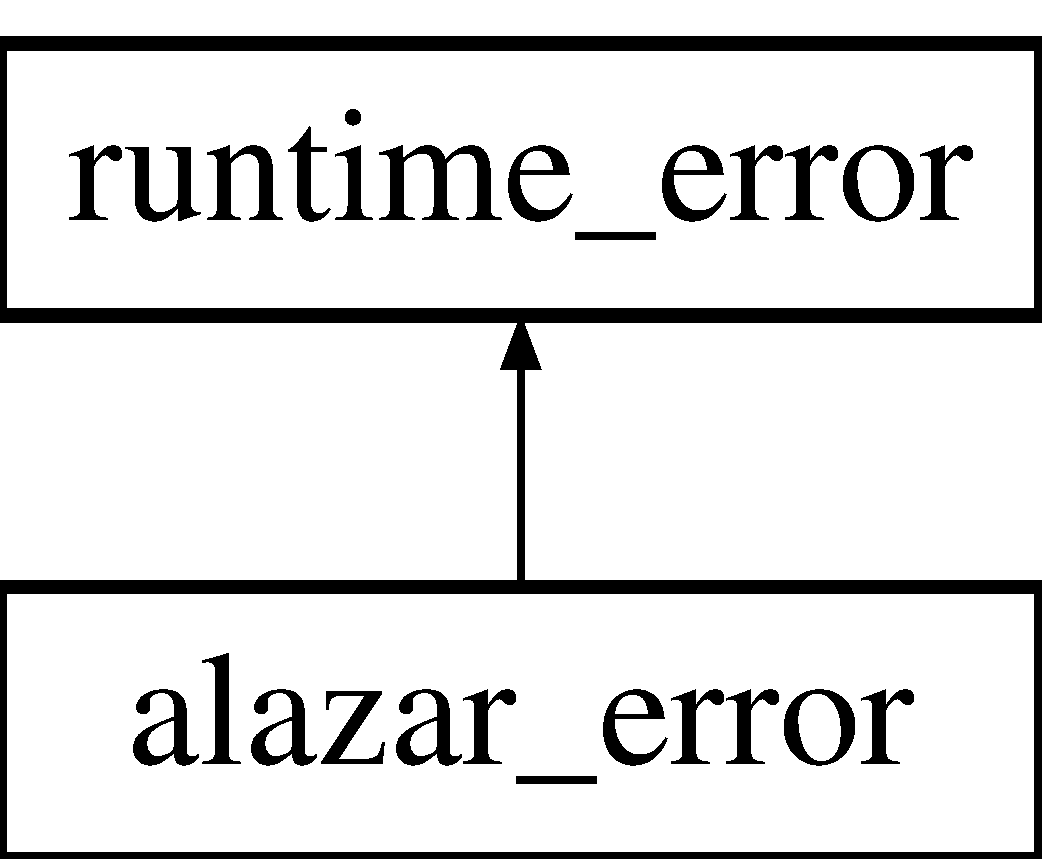
\includegraphics[height=2.000000cm]{classalazar__error}
\end{center}
\end{figure}
\subsection*{Public Member Functions}
\begin{DoxyCompactItemize}
\item 
{\bfseries alazar\+\_\+error} (R\+E\+T\+U\+R\+N\+\_\+\+C\+O\+DE ret)\hypertarget{classalazar__error_a762da54dc850295e0d06cbcd4ca0c02c}{}\label{classalazar__error_a762da54dc850295e0d06cbcd4ca0c02c}

\item 
virtual const char $\ast$ {\bfseries what} () const   throw ()\hypertarget{classalazar__error_a4aea33558f69d777c9d383c844021ddd}{}\label{classalazar__error_a4aea33558f69d777c9d383c844021ddd}

\item 
int {\bfseries Get\+Err\+Code} () const \hypertarget{classalazar__error_ac759f6b1f2eeb82daa2861ec10b875ad}{}\label{classalazar__error_ac759f6b1f2eeb82daa2861ec10b875ad}

\end{DoxyCompactItemize}

\hypertarget{classalazar_1_1_a_t_s9462}{}\section{alazar\+:\+:A\+T\+S9462 Class Reference}
\label{classalazar_1_1_a_t_s9462}\index{alazar\+::\+A\+T\+S9462@{alazar\+::\+A\+T\+S9462}}
Inheritance diagram for alazar\+:\+:A\+T\+S9462\+:\begin{figure}[H]
\begin{center}
\leavevmode
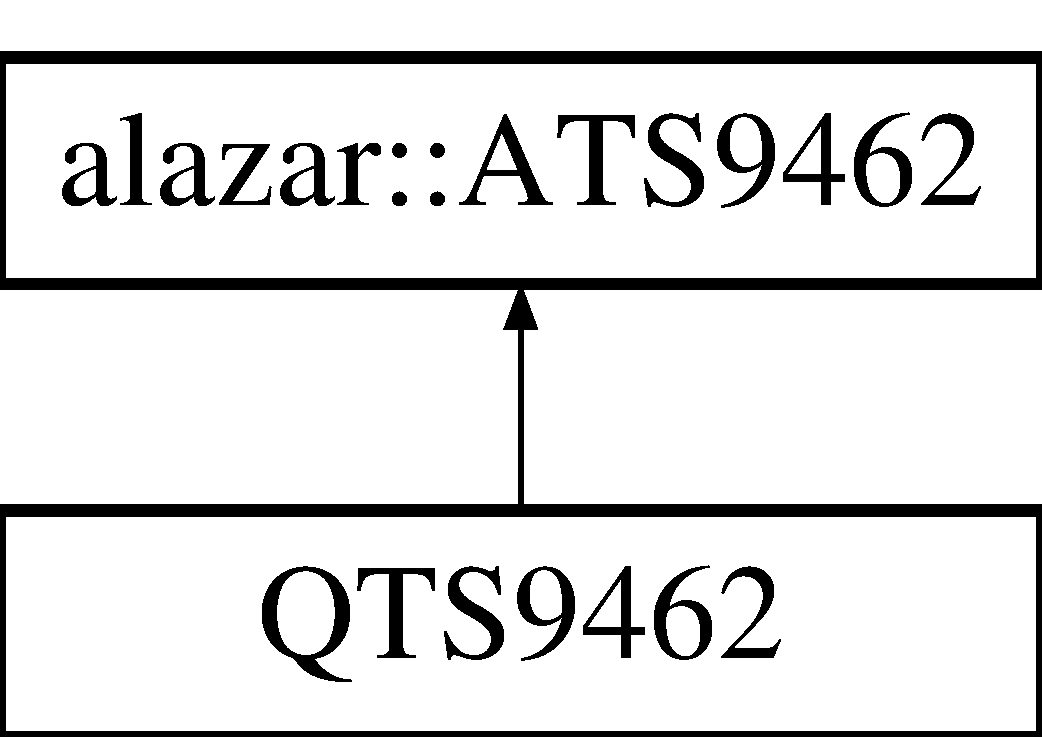
\includegraphics[height=2.000000cm]{classalazar_1_1_a_t_s9462}
\end{center}
\end{figure}
\subsection*{Public Types}
\begin{DoxyCompactItemize}
\item 
typedef std\+::lock\+\_\+guard$<$ std\+::mutex $>$ {\bfseries lock}\hypertarget{classalazar_1_1_a_t_s9462_a735d1f33b2ef63beda54f2d8bde5fd65}{}\label{classalazar_1_1_a_t_s9462_a735d1f33b2ef63beda54f2d8bde5fd65}

\end{DoxyCompactItemize}
\subsection*{Public Member Functions}
\begin{DoxyCompactItemize}
\item 
{\bfseries A\+T\+S9462} (uint system\+\_\+id=1, uint board\+\_\+id=1)\hypertarget{classalazar_1_1_a_t_s9462_a3c9661f8a645ad7decec5a88d000ac4b}{}\label{classalazar_1_1_a_t_s9462_a3c9661f8a645ad7decec5a88d000ac4b}

\item 
void {\bfseries Set\+Default\+Config} ()\hypertarget{classalazar_1_1_a_t_s9462_a105294c25a46cd9ccdefde67f939ebd2}{}\label{classalazar_1_1_a_t_s9462_a105294c25a46cd9ccdefde67f939ebd2}

\item 
std\+::vector$<$ short unsigned int $>$ {\bfseries Pull\+Raw\+Data} (uint data\+\_\+size)\hypertarget{classalazar_1_1_a_t_s9462_a36c812b7947f0747e956be07a1abc06b}{}\label{classalazar_1_1_a_t_s9462_a36c812b7947f0747e956be07a1abc06b}

\item 
std\+::vector$<$ double $>$ {\bfseries Pull\+Voltage\+Data} (uint data\+\_\+size)\hypertarget{classalazar_1_1_a_t_s9462_ab5b939ed5c26c0090167ba1a362410e9}{}\label{classalazar_1_1_a_t_s9462_ab5b939ed5c26c0090167ba1a362410e9}

\item 
std\+::vector$<$ double $>$ {\bfseries Pull\+Power\+Data} (uint data\+\_\+size)\hypertarget{classalazar_1_1_a_t_s9462_af3b77c6e5fec6305d86ea2e51079fca5}{}\label{classalazar_1_1_a_t_s9462_af3b77c6e5fec6305d86ea2e51079fca5}

\item 
void {\bfseries Select\+Channel} (Channel selection)\hypertarget{classalazar_1_1_a_t_s9462_a14212eb00bd058e6544e24538a77f485}{}\label{classalazar_1_1_a_t_s9462_a14212eb00bd058e6544e24538a77f485}

\item 
void {\bfseries Set\+Capture\+Clock} ()\hypertarget{classalazar_1_1_a_t_s9462_abff5593d1a4186e575b440cb48a61130}{}\label{classalazar_1_1_a_t_s9462_abff5593d1a4186e575b440cb48a61130}

\item 
void {\bfseries Input\+Control\+ChannelA} ()\hypertarget{classalazar_1_1_a_t_s9462_a5eab01e620a5eb08aaa9a1109c55b130}{}\label{classalazar_1_1_a_t_s9462_a5eab01e620a5eb08aaa9a1109c55b130}

\item 
void {\bfseries Input\+Control\+ChannelB} ()\hypertarget{classalazar_1_1_a_t_s9462_ab9879af3916cde958d9b93fd16211acc}{}\label{classalazar_1_1_a_t_s9462_ab9879af3916cde958d9b93fd16211acc}

\item 
void {\bfseries Set\+B\+W\+Limit} ()\hypertarget{classalazar_1_1_a_t_s9462_a5153f8e7f52791b42f9b1bbd736df07b}{}\label{classalazar_1_1_a_t_s9462_a5153f8e7f52791b42f9b1bbd736df07b}

\item 
void {\bfseries Set\+Trigger\+Operation} ()\hypertarget{classalazar_1_1_a_t_s9462_a84a882e5493371b9b57342fcc87d6ee2}{}\label{classalazar_1_1_a_t_s9462_a84a882e5493371b9b57342fcc87d6ee2}

\item 
void {\bfseries Set\+External\+Trigger} ()\hypertarget{classalazar_1_1_a_t_s9462_af0e0cfb35e881334d938e4855fe0076b}{}\label{classalazar_1_1_a_t_s9462_af0e0cfb35e881334d938e4855fe0076b}

\item 
void {\bfseries Set\+Trigger\+Time\+Out} (double trigger\+\_\+timerout\+\_\+sec=0.\+0f)\hypertarget{classalazar_1_1_a_t_s9462_a1072b3409870b3f41ed8ac43eb5bc45f}{}\label{classalazar_1_1_a_t_s9462_a1072b3409870b3f41ed8ac43eb5bc45f}

\item 
void {\bfseries Configure\+Aux\+IO} ()\hypertarget{classalazar_1_1_a_t_s9462_a677ccd33c37a38bc7a89e05af03248b8}{}\label{classalazar_1_1_a_t_s9462_a677ccd33c37a38bc7a89e05af03248b8}

\item 
void {\bfseries Set\+Integration\+Time} (double time\+\_\+sec)\hypertarget{classalazar_1_1_a_t_s9462_a772c256adaf6cbe6fde92ec85c69bf74}{}\label{classalazar_1_1_a_t_s9462_a772c256adaf6cbe6fde92ec85c69bf74}

\item 
void {\bfseries Set\+Sample\+Rate} (double samples\+\_\+per\+\_\+sec)\hypertarget{classalazar_1_1_a_t_s9462_a474ca0033e639f167d8fc0c19016ae38}{}\label{classalazar_1_1_a_t_s9462_a474ca0033e639f167d8fc0c19016ae38}

\item 
void {\bfseries Start\+Capture} ()\hypertarget{classalazar_1_1_a_t_s9462_a7efd31862655888e14aacaaed0bf7b66}{}\label{classalazar_1_1_a_t_s9462_a7efd31862655888e14aacaaed0bf7b66}

\item 
void {\bfseries Abort\+Capture} ()\hypertarget{classalazar_1_1_a_t_s9462_acea0e4b18a527d16eded70af1ebb32f2}{}\label{classalazar_1_1_a_t_s9462_acea0e4b18a527d16eded70af1ebb32f2}

\end{DoxyCompactItemize}
\subsection*{Protected Attributes}
\begin{DoxyCompactItemize}
\item 
u\+\_\+char {\bfseries bits\+\_\+per\+\_\+sample}\hypertarget{classalazar_1_1_a_t_s9462_a3c06879f4a472cae8980dbca59de2ab8}{}\label{classalazar_1_1_a_t_s9462_a3c06879f4a472cae8980dbca59de2ab8}

\item 
uint {\bfseries max\+\_\+samples\+\_\+per\+\_\+channel}\hypertarget{classalazar_1_1_a_t_s9462_a35fb6e0f8229d283a7cf5a3caa019477}{}\label{classalazar_1_1_a_t_s9462_a35fb6e0f8229d283a7cf5a3caa019477}

\item 
uint {\bfseries bytes\+\_\+per\+\_\+buffer} = 0\hypertarget{classalazar_1_1_a_t_s9462_acf368609145cef04df523fd4e4dc3e3f}{}\label{classalazar_1_1_a_t_s9462_acf368609145cef04df523fd4e4dc3e3f}

\item 
uint {\bfseries buffers\+\_\+per\+\_\+acquisition} = 0\hypertarget{classalazar_1_1_a_t_s9462_a9edef52c0c4cd04f2d10e4c70abf5846}{}\label{classalazar_1_1_a_t_s9462_a9edef52c0c4cd04f2d10e4c70abf5846}

\item 
uint {\bfseries buffer\+\_\+count} = 4\hypertarget{classalazar_1_1_a_t_s9462_a564b69f9a510c11797498646cefd34a1}{}\label{classalazar_1_1_a_t_s9462_a564b69f9a510c11797498646cefd34a1}

\item 
uint {\bfseries samples\+\_\+per\+\_\+buffer} = 204800\hypertarget{classalazar_1_1_a_t_s9462_ac88e42e562a19d5a85854d2141652bad}{}\label{classalazar_1_1_a_t_s9462_ac88e42e562a19d5a85854d2141652bad}

\item 
double {\bfseries integration\+\_\+time} = 0.\+0f\hypertarget{classalazar_1_1_a_t_s9462_a089bac3e1e8014fbdf632839b7f31bd3}{}\label{classalazar_1_1_a_t_s9462_a089bac3e1e8014fbdf632839b7f31bd3}

\item 
double {\bfseries sample\+\_\+rate} = 0.\+0f\hypertarget{classalazar_1_1_a_t_s9462_a68dd5fc314dfc932a9f3dd50c7cdc117}{}\label{classalazar_1_1_a_t_s9462_a68dd5fc314dfc932a9f3dd50c7cdc117}

\item 
uint {\bfseries ring\+\_\+buffer\+\_\+size} = 1e6\hypertarget{classalazar_1_1_a_t_s9462_a6b25da2772535b5424e2131e01c95fd6}{}\label{classalazar_1_1_a_t_s9462_a6b25da2772535b5424e2131e01c95fd6}

\end{DoxyCompactItemize}

\hypertarget{classjaspl_1_1j_spectrum_analyzer}{}\section{jaspl\+:\+:j\+Spectrum\+Analyzer Class Reference}
\label{classjaspl_1_1j_spectrum_analyzer}\index{jaspl\+::j\+Spectrum\+Analyzer@{jaspl\+::j\+Spectrum\+Analyzer}}
Inheritance diagram for jaspl\+:\+:j\+Spectrum\+Analyzer\+:\begin{figure}[H]
\begin{center}
\leavevmode
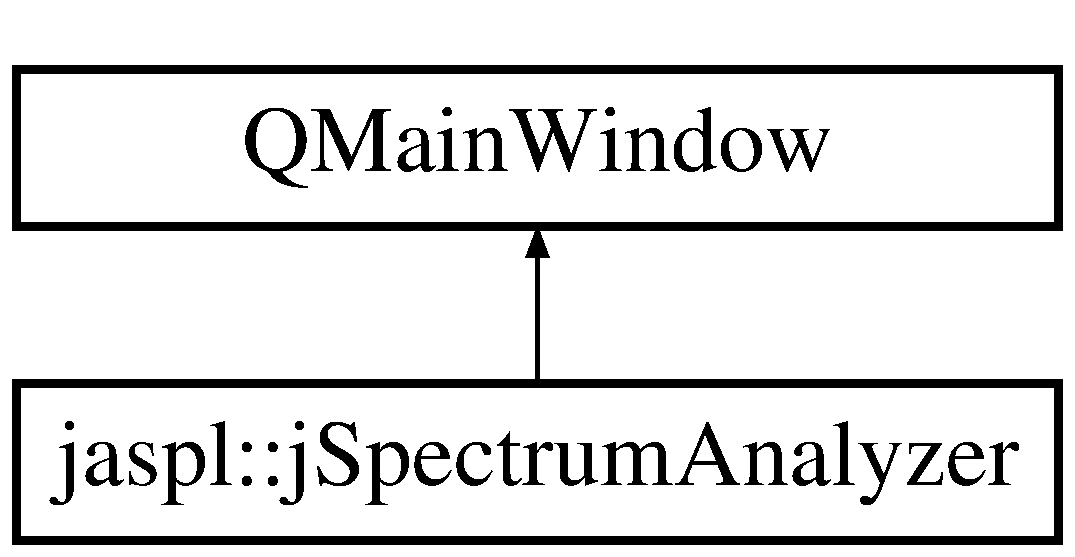
\includegraphics[height=2.000000cm]{classjaspl_1_1j_spectrum_analyzer}
\end{center}
\end{figure}
\subsection*{Public Slots}
\begin{DoxyCompactItemize}
\item 
void {\bfseries Update\+Signal} (std\+::vector$<$ double $>$ time\+\_\+series, uint sample\+\_\+rate)\hypertarget{classjaspl_1_1j_spectrum_analyzer_a0724baa59176c7e8a0050f52472f578f}{}\label{classjaspl_1_1j_spectrum_analyzer_a0724baa59176c7e8a0050f52472f578f}

\end{DoxyCompactItemize}
\subsection*{Signals}
\begin{DoxyCompactItemize}
\item 
void {\bfseries Signal\+Changed} ()\hypertarget{classjaspl_1_1j_spectrum_analyzer_a9c5cf1221b35e6392fff8bf418edcedd}{}\label{classjaspl_1_1j_spectrum_analyzer_a9c5cf1221b35e6392fff8bf418edcedd}

\end{DoxyCompactItemize}
\subsection*{Public Member Functions}
\begin{DoxyCompactItemize}
\item 
{\bfseries j\+Spectrum\+Analyzer} (Q\+Widget $\ast$parent=0)\hypertarget{classjaspl_1_1j_spectrum_analyzer_a5101faac87201a91ea02e2afcbdf33db}{}\label{classjaspl_1_1j_spectrum_analyzer_a5101faac87201a91ea02e2afcbdf33db}

\item 
void {\bfseries Activate} ()\hypertarget{classjaspl_1_1j_spectrum_analyzer_a778e2eef7d689c8b9f4df3d0894af4a2}{}\label{classjaspl_1_1j_spectrum_analyzer_a778e2eef7d689c8b9f4df3d0894af4a2}

\item 
{\footnotesize template$<$class T , typename F $>$ }\\void {\bfseries Plot} (T y\+\_\+signal\+\_\+elements, F x\+\_\+frequency\+\_\+range)\hypertarget{classjaspl_1_1j_spectrum_analyzer_a1a9a7d7efd93e37a1bd76a7123cf4caf}{}\label{classjaspl_1_1j_spectrum_analyzer_a1a9a7d7efd93e37a1bd76a7123cf4caf}

\item 
{\footnotesize template$<$class T , typename F $>$ }\\void {\bfseries Plot} (T y\+\_\+signal\+\_\+elements, F x\+\_\+frequency\+\_\+range, std\+::string chart\+\_\+title)\hypertarget{classjaspl_1_1j_spectrum_analyzer_aff0590acca8571ced9b05a6d0f7932fb}{}\label{classjaspl_1_1j_spectrum_analyzer_aff0590acca8571ced9b05a6d0f7932fb}

\end{DoxyCompactItemize}

\hypertarget{class_main_window}{}\section{Main\+Window Class Reference}
\label{class_main_window}\index{Main\+Window@{Main\+Window}}
Inheritance diagram for Main\+Window\+:\begin{figure}[H]
\begin{center}
\leavevmode
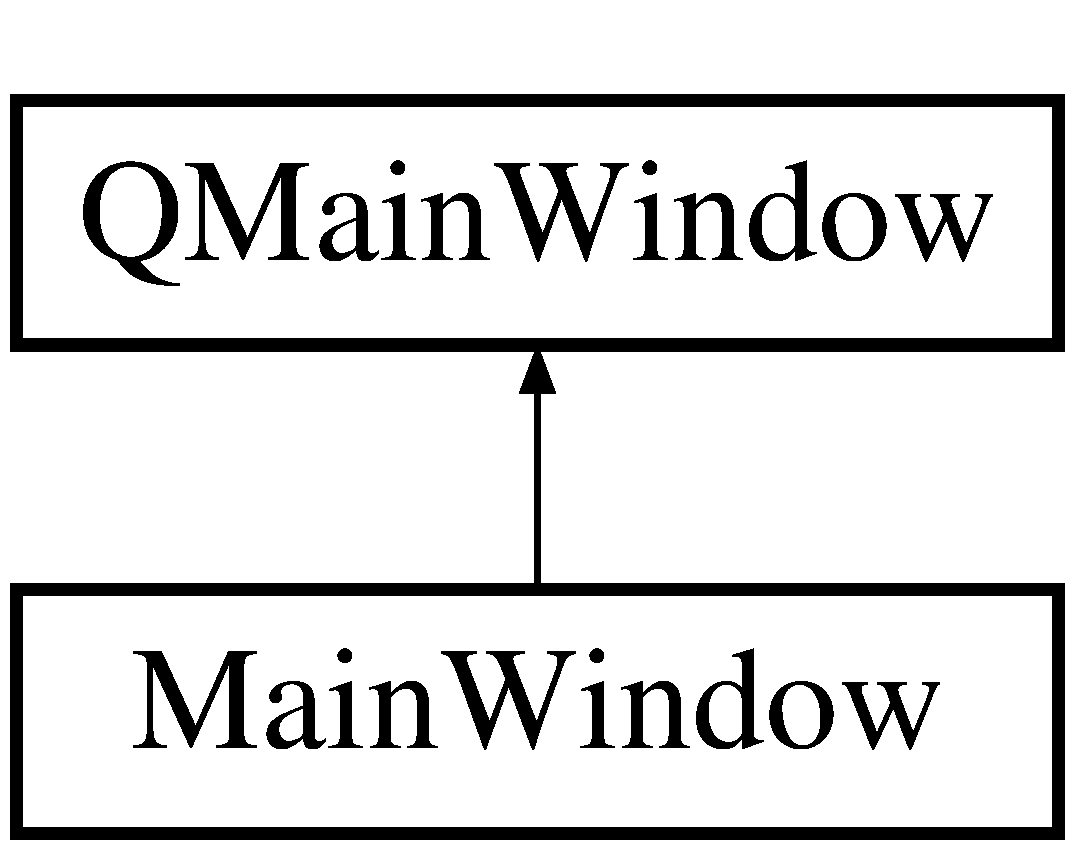
\includegraphics[height=2.000000cm]{class_main_window}
\end{center}
\end{figure}
\subsection*{Public Member Functions}
\begin{DoxyCompactItemize}
\item 
{\bfseries Main\+Window} (Q\+Widget $\ast$parent=0)\hypertarget{class_main_window_a8b244be8b7b7db1b08de2a2acb9409db}{}\label{class_main_window_a8b244be8b7b7db1b08de2a2acb9409db}

\end{DoxyCompactItemize}

\hypertarget{class_q_t_s9462}{}\section{Q\+T\+S9462 Class Reference}
\label{class_q_t_s9462}\index{Q\+T\+S9462@{Q\+T\+S9462}}
Inheritance diagram for Q\+T\+S9462\+:\begin{figure}[H]
\begin{center}
\leavevmode
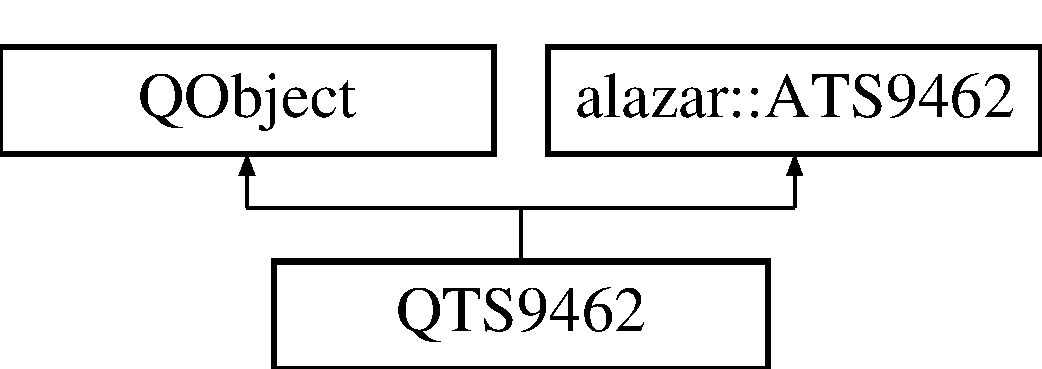
\includegraphics[height=2.000000cm]{class_q_t_s9462}
\end{center}
\end{figure}
\subsection*{Public Slots}
\begin{DoxyCompactItemize}
\item 
void {\bfseries Update\+Samples\+Sent} (uint num\+\_\+samples)\hypertarget{class_q_t_s9462_a4f8594f3594d17bc620f461940b9c363}{}\label{class_q_t_s9462_a4f8594f3594d17bc620f461940b9c363}

\item 
void {\bfseries Send\+Time\+Series} ()\hypertarget{class_q_t_s9462_a8ebb7837f39380fa67e3d206de57d332}{}\label{class_q_t_s9462_a8ebb7837f39380fa67e3d206de57d332}

\item 
void {\bfseries Start} ()\hypertarget{class_q_t_s9462_a3d47467dc91daadd830b52259dde71ab}{}\label{class_q_t_s9462_a3d47467dc91daadd830b52259dde71ab}

\item 
void {\bfseries Stop} ()\hypertarget{class_q_t_s9462_af1fac33559f85b79918e7b74aecb1e0c}{}\label{class_q_t_s9462_af1fac33559f85b79918e7b74aecb1e0c}

\end{DoxyCompactItemize}
\subsection*{Signals}
\begin{DoxyCompactItemize}
\item 
void {\bfseries Raw\+Time\+Series} (std\+::vector$<$ short unsigned int $>$ time\+\_\+series, uint s\+\_\+rate)\hypertarget{class_q_t_s9462_a0c2f091b771c1737a9d217206cb3db1d}{}\label{class_q_t_s9462_a0c2f091b771c1737a9d217206cb3db1d}

\item 
void {\bfseries Voltage\+Time\+Series} (std\+::vector$<$ double $>$ time\+\_\+series, uint s\+\_\+rate)\hypertarget{class_q_t_s9462_a0b89d044f501bb3ccde93f6c95235247}{}\label{class_q_t_s9462_a0b89d044f501bb3ccde93f6c95235247}

\end{DoxyCompactItemize}
\subsection*{Public Member Functions}
\begin{DoxyCompactItemize}
\item 
{\bfseries Q\+T\+S9462} (Q\+Object $\ast$parent=0, uint system\+\_\+id=1, uint board\+\_\+id=1)\hypertarget{class_q_t_s9462_a593b946f814029a41a2efe72e6a91b48}{}\label{class_q_t_s9462_a593b946f814029a41a2efe72e6a91b48}

\end{DoxyCompactItemize}
\subsection*{Additional Inherited Members}

%--- End generated contents ---

% Index
\backmatter
\newpage
\phantomsection
\clearemptydoublepage
\addcontentsline{toc}{chapter}{Index}
\printindex

\end{document}
